\documentclass[11pt]{article}

\usepackage[letterpaper,margin=1in]{geometry}
\usepackage{microtype}
\usepackage{amsmath}
\usepackage{amssymb}
\usepackage{booktabs}
\usepackage{array}
\usepackage[table,dvipsnames]{xcolor}
\usepackage{enumitem}
\usepackage{tikz}
\usetikzlibrary{positioning,arrows.meta,shapes.geometric,fit,backgrounds,calc}
\usepackage[most]{tcolorbox}
\usepackage{float}
\usepackage[hidelinks]{hyperref}

\emergencystretch=3em  % absorb the occasional unbreakable prose line

% Plain-language callout: a non-technical summary readers can rely on without
% reading the math around it.
\newtcolorbox{plain}{
  enhanced, breakable,
  colback=Sepia!7, colframe=Sepia!55, boxrule=0.4pt, arc=2pt,
  left=7pt, right=7pt, top=4pt, bottom=4pt,
  fontupper=\small,
  coltitle=Sepia!72!black, fonttitle=\bfseries\sffamily\footnotesize,
  title={IN PLAIN TERMS}
}

% --- palette ---
\definecolor{crit}{HTML}{C0392B}
\definecolor{high}{HTML}{E67E22}
\definecolor{med}{HTML}{F1C40F}
\definecolor{low}{HTML}{27AE60}
\definecolor{infoblue}{HTML}{2C3E50}
\definecolor{tagbg}{HTML}{ECF0F1}
\definecolor{rule}{HTML}{BDC3C7}

\newcommand{\tagn}[1]{{\footnotesize\ttfamily #1}}
\newcommand{\code}[1]{\texttt{#1}}
\newcommand{\rfckw}[1]{\textsc{#1}}

\title{\bfseries A Deterministic, CVSS--Environmental Method for\\
FedRAMP Rev5 VDR/VER Vulnerability Prioritization}
\author{stackArmor \\ \small Draft Whitepaper / Request for Comments}
\date{June 2026 \quad\textbar\quad Status: Informational Draft}

\begin{document}
\maketitle

\begin{abstract}
\noindent
FedRAMP Rev5 introduces a Vulnerability Disclosure Report (VDR) and Vulnerability
Evaluation Requirements (VER) that define \emph{Potential Agency Impact} (PAIN,
levels N1--N5) and a remediation--timeframe matrix, together with evaluation rules
for likely exploitability and internet reachability. FedRAMP deliberately does
\emph{not} prescribe how to derive a PAIN level from an individual vulnerability on
a specific asset. This memo argues that the missing classifier already exists, in
standardized form, as the \textbf{Environmental metric group of CVSS}: the
Confidentiality, Integrity and Availability \emph{Requirements} (CR/IR/AR) and the
Modified Impact Sub-Score were designed precisely to re-weight a vulnerability's
impact by what is at stake in a given deployment. We present a closed-form,
reproducible mapping from FedRAMP's requirements onto CVSS Environmental metrics,
derive PAIN and the remediation deadline from it, and give fully worked
calculations. We also present an \emph{example} mechanism --- ``asset archetypes''
--- for assigning CR/IR/AR systematically, while emphasizing that each Cloud Service
Provider (CSP) \rfckw{should} derive its own assignment from its system
categorization. A reference architecture and a sample scan complete the memo.
\end{abstract}

\tableofcontents

\section{Status of This Memo and Terminology}
This document is an informational draft circulated for comment. It does not define
a FedRAMP requirement; it proposes a standardized \emph{method} for satisfying
existing VDR/VER requirements.

The key words \rfckw{must}, \rfckw{must not}, \rfckw{should}, \rfckw{should not},
and \rfckw{may} are to be interpreted as described in RFC~2119.

\begin{description}[leftmargin=1.5em,style=nextline]
\item[PAIN] Potential Agency Impact, the FedRAMP N1--N5 rating of a finding.
\item[CR/IR/AR] The CVSS Environmental Confidentiality / Integrity / Availability
  \emph{Requirements} of an asset.
\item[ISC] Impact Sub-Score (here, the CVSS \emph{Modified} Impact Sub-Score).
\item[LEV / NLEV] Likely Exploitable / Not Likely Exploitable (a VER axis).
\item[IRV / NIRV] Internet Reachable / Not Internet Reachable (a VER axis).
\item[Class] The provider Certification Class (A--D) selecting a remediation table.
\end{description}

\section{Motivation: the gap between VDR/VER and the scanner}
\begin{plain}
A scanner tells you a flaw exists and how severe it is \emph{in the abstract}.
FedRAMP asks a different question: how bad is this flaw \emph{for the agency}, on
\emph{this exact system}, and how fast must we fix it? A ``low''-rated flaw on the
database holding everyone's records can matter more than a ``high'' on a throwaway
test box. This memo gives one consistent, repeatable way to answer FedRAMP's
question --- instead of leaving it to each analyst's judgment.
\end{plain}
A vulnerability scanner emits, per finding, a CVE identifier, a qualitative
severity, and (often) a CVSS Base vector. FedRAMP Rev5 VDR/VER, by contrast, asks
the provider to answer a different question: \emph{what is the potential impact on
the agency if this vulnerability is exploited on this asset, and how quickly must
it therefore be remediated?} The two are not the same. A ``Low''-rated CVE on a
crown-jewel datastore can carry more agency impact than a ``High''-rated CVE on a
throwaway sandbox.

FedRAMP supplies the \emph{output} vocabulary (the PAIN buckets and the remediation
matrix) and the \emph{evaluation axes} (likely-exploitable, internet-reachable) but
leaves the \emph{classifier} --- the function from (CVE, asset) to PAIN --- to the
provider. An ad-hoc or analyst-by-analyst classifier is neither reproducible nor
defensible. This memo supplies a deterministic one.

\section{Key insight: FedRAMP's requirements are CVSS Environmental metrics}
\begin{plain}
You don't need a brand-new risk formula. The industry-standard CVSS scoring system
already has a built-in way to say ``this system is especially critical, so weight
its flaws more heavily.'' That built-in knob is exactly what FedRAMP's ``impact on
the agency'' is asking for. We simply turn the knob on, instead of inventing
something new.
\end{plain}
The central claim of this memo is that FedRAMP's notion of ``impact on the agency''
maps, almost one-to-one, onto metrics that already exist in the CVSS v3.1
specification's \emph{Environmental} group. The Environmental group exists for
exactly this purpose: to let the consuming organization re-score a vulnerability
according to the criticality of the affected asset in \emph{its} environment.

\begin{table}[H]
\centering
\renewcommand{\arraystretch}{1.25}
\begin{tabular}{>{\raggedright\arraybackslash}p{0.44\textwidth} >{\raggedright\arraybackslash}p{0.44\textwidth}}
\toprule
\textbf{FedRAMP VDR/VER concept} & \textbf{CVSS mechanism that satisfies it} \\
\midrule
Asset data sensitivity / FIPS-199 C-I-A categorization & Security Requirements
\code{CR}, \code{IR}, \code{AR} \\
Magnitude of potential agency impact & Modified Impact Sub-Score (\code{ISC}) \\
Likely exploitable (VER) & \code{LEV}: exploit maturity (CISA Vulnrichment) / EPSS threshold \\
Internet reachable (VER) & \code{IRV}: deployment/network context \\
Single- vs.\ multi-agency blast radius & scope multiplier on the PAIN tier \\
Provider Certification Class & selector of the remediation deadline table \\
\bottomrule
\end{tabular}
\caption{FedRAMP requirements fall directly onto CVSS Environmental metrics.}
\end{table}

The consequence is that a conforming implementation need not invent a bespoke
risk algebra. It need only (a) assign each asset its CR/IR/AR, and (b) evaluate the
two VER axes. The arithmetic that turns those inputs into a defensible impact
magnitude is the published CVSS Environmental formula.

\section{The model}
\begin{plain}
Two questions decide everything. (1)~\textbf{How much damage} could this flaw do to
\emph{this} system? (2)~Does the system hold \textbf{one agency's} data or
\textbf{many}? Question~1 produces a word --- Minimal, Narrow, Disruptive, or
Debilitating. Question~2 decides whether a ``Disruptive'' or ``Debilitating'' result
counts once or is escalated because several agencies are exposed. Together they pick
the final N1--N5 level.
\end{plain}
We define PAIN as a function of a \emph{severity} term and a \emph{scope} term:
\[
\text{PAIN}(\text{finding}) \;=\; f\big(\,\text{SEVERITY},\ \text{SCOPE}\,\big).
\]
\textbf{SEVERITY} answers ``how badly does this vulnerability's impact land on
\emph{this} asset?'' --- the CVE's impact metrics re-weighted by the asset's
CR/IR/AR. \textbf{SCOPE} answers ``how many agencies' data does the asset hold?''
--- single (1) or multiple ($>1$). SEVERITY is mapped to a FedRAMP customer-effect
word (Minimal, Narrow, Disruptive, Debilitating); the word and scope together
select the N-level.

\section{Two threat inputs from CISA Vulnrichment}
\label{sec:enrichment}
\begin{plain}
Beyond the CVE's own CVSS vector, the method pulls in two facts about each flaw from
\emph{CISA Vulnrichment} --- CISA's Authorized Data Publisher (ADP) enrichment of CVE
records: how the flaw is actually being exploited, and how much control exploitation
grants. One tightens the remediation \emph{clock}; the other can raise the PAIN
\emph{level}. Both are optional: without them the method falls back to the CVSS vector
and EPSS alone.
\end{plain}

Two distinct inputs feed two distinct stages:
\begin{itemize}[leftmargin=1.4em]
\item \textbf{Exploitation state} (active / PoC / none) $\rightarrow$ the
  \textbf{remediation clock}. ``active'' makes a finding Likely Exploitable (LEV)
  regardless of its EPSS probability, moving it to a faster remediation column
  (Section~\ref{sec:remediation}).
\item \textbf{Technical impact} (total / partial) $\rightarrow$ the \textbf{PAIN
  level}. ``total'' floors the in-scope CVSS impact to High before the CR/IR/AR
  weighting, which can push a finding up a tier (Section~\ref{sec:math}).
\end{itemize}

\noindent How it plays in --- three quick illustrations (Class~C, single-agency):
\begin{itemize}[leftmargin=1.4em]
\item \emph{Exploitation moves the clock.} An N3 finding with EPSS $0.30$ (below
  threshold) sits in the slow column: \textbf{128 days}. Mark it
  \code{exploitation = active} and it becomes LEV --- the deadline drops to
  \textbf{16 days} (internet-reachable) or 32 days (not).
\item \emph{Technical impact moves the level.} A ``weak'' RCE (low impact across
  C/I/A) on a High/High/High asset scores Disruptive $\rightarrow$ \textbf{N3}. Mark
  it \code{technical impact = total} and the in-scope dimensions floor to High,
  scoring Debilitating $\rightarrow$ \textbf{N4} (worked in Example~5).
\item \emph{Neither present.} No active exploitation, sub-threshold EPSS, and
  partial/absent technical impact $\rightarrow$ the finding is scored purely on its
  CVSS vector and stays in the slow column at its base tier.
\end{itemize}

\section{The mathematics}
\label{sec:math}
\begin{plain}
This is the engine room --- you can skim the equations and still follow the idea.
Every flaw can hurt three things: \textbf{secrecy}, \textbf{correctness}, and
\textbf{uptime}. For each, we multiply ``how badly the flaw breaks it'' by ``how much
this system depends on it,'' then combine the three into a single damage score
between 0 and 1. Finally we translate that score into a plain word. Bigger number =
more damage. The only place human judgment enters is the three cut-points that decide
where one word becomes the next.
\end{plain}
All constants below are taken \emph{verbatim} from the CVSS v3.1 specification; only
the normalization and the word thresholds (Section~\ref{sec:thresholds}) are
additions.

\begin{plain}
\textbf{What the symbols mean.}
\begin{itemize}[leftmargin=1.3em,nosep,topsep=2pt]
\item $C, I, A$ --- how badly \emph{this flaw} breaks secrecy, correctness, and
  uptime (from the CVE's CVSS vector). None / Low / High become $0$ / $0.22$ / $0.56$.
\item $\mathrm{CR},\mathrm{IR},\mathrm{AR}$ --- how much \emph{this system} needs
  secrecy, correctness, and uptime (from its archetype). Low / Medium / High become
  $0.5$ / $1.0$ / $1.5$.
\item $\mathrm{ISC}$ --- the three combined into one ``damage to this system'' number.
\item $S$ --- that damage rescaled to a clean $0$--$1$ range.
\item $W$ --- the plain English word $S$ maps to.
\item $m$ --- does the system serve one agency ($0$) or many ($1$)? Resolved
  hierarchically from the workload/namespace/cluster tags.
\item $\theta_1,\theta_2,\theta_3$ --- the three cut-points where the word changes.
\end{itemize}
\end{plain}

\paragraph{Impact metric weights.}
Each of the affected vulnerability's Confidentiality, Integrity and Availability
impact metrics ($C$, $I$, $A$), read from the CVSS Base vector, takes a weight:
\[
C, I, A \in \{\,\text{None}=0,\quad \text{Low}=0.22,\quad \text{High}=0.56\,\}.
\]

\paragraph{Security Requirement weights.}
Each asset's Requirement (CR, IR, AR) takes a multiplier:
\[
\mathrm{CR},\mathrm{IR},\mathrm{AR} \in \{\,\text{Low}=0.5,\quad \text{Medium}=1.0,\quad \text{High}=1.5\,\}.
\]

\paragraph{Modified Impact Sub-Score.}
The per-dimension impacts and requirements combine as a probabilistic union --- the
share of the asset left uncompromised on each dimension is multiplied, and the
complement is the overall impact:
\begin{equation}
\mathrm{ISC} \;=\; \min\!\Big[\,1 - \big(1 - C\!\cdot\!\mathrm{CR}\big)\big(1 - I\!\cdot\!\mathrm{IR}\big)\big(1 - A\!\cdot\!\mathrm{AR}\big),\ \ 0.915\,\Big].
\label{eq:isc}
\end{equation}
The cap $0.915 = 1-(1-0.56)^3$ is the CVSS ceiling (all-High impact at Medium
requirements). We then normalize to a unit scalar:
\begin{equation}
S \;=\; \frac{\mathrm{ISC}}{0.915} \ \in\ [0,1].
\label{eq:s}
\end{equation}

\paragraph{Severity word.}
\label{sec:thresholds}
$S$ is bucketed into a FedRAMP customer-effect word by three cut points
$(\theta_1,\theta_2,\theta_3)$:
\begin{equation}
W(S) \;=\;
\begin{cases}
\text{Minimal} & S < \theta_1 \\
\text{Narrow} & \theta_1 \le S < \theta_2 \\
\text{Disruptive} & \theta_2 \le S < \theta_3 \\
\text{Debilitating} & S \ge \theta_3
\end{cases}
\qquad (\theta_1,\theta_2,\theta_3) = (0.25,\ 0.55,\ 0.80).
\label{eq:word}
\end{equation}
The cut points are the model's \emph{one} calibratable judgment. They
\rfckw{should} be documented and back-tested against analyst-rated findings, and an
implementation \rfckw{must} treat them as governed configuration rather than an
in-band, ad-hoc setting.

\paragraph{Scope and the N-level.}
Let $m \in \{0,1\}$ be the asset's multi-agency flag, resolved most-specific-first:
workload label, then namespace label, then a namespace glob, then the cluster
default (Section~\ref{sec:archetypes}). Scope is purely hierarchical --- an asset is
multi-agency only if it (or its namespace, or the cluster) is tagged so. The N-level
follows from the word and scope:
\begin{equation}
\text{PAIN} =
\begin{cases}
\text{N1} & W=\text{Minimal} \\
\text{N2} & W=\text{Narrow} \\
\text{N3} & W=\text{Disruptive},\ m=0 \\
\text{N4} & W=\text{Disruptive},\ m=1 \ \ \text{or}\ \ W=\text{Debilitating},\ m=0 \\
\text{N5} & W=\text{Debilitating},\ m=1
\end{cases}
\label{eq:pain}
\end{equation}

\paragraph{Technical-impact floor (optional refinement).}
Where an authoritative source (e.g.\ CISA Vulnrichment SSVC) provides a
\emph{technical impact} of \code{total}, the impacts that the CVE \emph{does} touch
may be floored to High before Eq.~\eqref{eq:isc}:
\[
\hat{X} = \begin{cases} 0.56 & X>0 \ \text{and}\ \text{tech.\ impact}=\code{total} \\ X & \text{otherwise} \end{cases}
\qquad X \in \{C,I,A\}.
\]
Crucially the floor \rfckw{must not} invent impact on a dimension the CVE marks
None ($X=0$ stays $0$); \code{partial} or absent leaves the vector unchanged.

\section{Fail-safe behavior}
\begin{plain}
If a system hasn't been classified yet, we assume the worst, not the best --- it
scores high and shows up loudly until someone classifies it. Silence never makes a
problem look smaller than it is.
\end{plain}
Missing metadata \rfckw{must not} \emph{lower} PAIN. An asset that carries no
classification \rfckw{should} resolve to a deliberately conservative default
(e.g.\ CR/IR/AR all High), which scores loudly and surfaces the asset for
classification rather than hiding it. ``Unknown'' is treated as ``serious until
proven otherwise.''

\section{Remediation: the VDR-TFR-PVR matrix}
\label{sec:remediation}
\begin{plain}
The N-level says \emph{how bad}; this step says \emph{how fast}. Two real-world facts
tighten the clock: is the flaw actually being exploited (or very likely to be), and
is the system reachable from the internet? More severe + more exploitable + more
exposed = less time to fix. A lookup table turns those into a concrete deadline,
stricter for higher-assurance providers.
\end{plain}
The remediation deadline is selected by three values: the provider Certification
Class, the PAIN level, and an exploitability \emph{column} derived from the two VER
axes:
\[
\text{deadline} = M\big[\,\text{Class}\,\big]\big[\,\text{PAIN}\,\big]\big[\,\text{column}\,\big],
\qquad
\text{column} \in \{\,\text{LEV+IRV},\ \text{LEV+NIRV},\ \text{NLEV}\,\}.
\]
where, for a provider-selected EPSS threshold $\theta_{\text{epss}}$ (this memo uses
$0.70$):
\[
\text{LEV} \;=\; \big(\text{EPSS} \ge \theta_{\text{epss}}\big)\ \lor\ \big(\text{exploitation} = \text{active}\big),
\qquad
\text{IRV} = \text{asset is internet-reachable}.
\]
Here \emph{internet-reachable} means the asset is fronted by a \textbf{public-facing
load balancer or route whose edge does not itself enforce authentication}. A route
gated by native edge authentication --- an identity-aware proxy or equivalent that
authenticates every request before it reaches the workload --- is treated as
\emph{not} internet-reachable (NIRV), on the view that an unauthenticated attacker
cannot reach the vulnerable surface. (How a given platform's routes and edge
authentication are discovered is an implementation concern, out of scope here.)

Both the exploitation state here and the technical impact in
Section~\ref{sec:math} are sourced from \emph{CISA Vulnrichment}, an Authorized Data
Publisher (ADP) in the CVE Program; that choice is itself a design opinion (see
Appendix~\ref{app:opinions}). The day-valued tables are given in
Appendix~\ref{app:matrix}. PAIN-1 carries no FedRAMP deadline.

\section{Worked examples}
\begin{plain}
The same formula, run by hand on realistic cases. Watch the \emph{same}
vulnerability land at very different N-levels depending only on which system it sits
on --- that is the entire point of the method.
\end{plain}
We use $C,I,A$ for impacts and CR/IR/AR for requirements; all arithmetic follows
Eqs.~\eqref{eq:isc}--\eqref{eq:pain}.

\paragraph{Example 1 --- RCE on a crown-jewel datastore, multi-agency.}
$C\!=\!I\!=\!A\!=\!0.56$ (High), CR=IR=AR=$1.5$ (High), $m=1$.
\begin{align*}
\mathrm{ISC} &= \min\!\big[\,1-(1-0.84)^3,\ 0.915\,\big] = \min[\,0.9959,\ 0.915\,] = 0.915, \\
S &= 0.915/0.915 = 1.000 \;\Rightarrow\; W=\text{Debilitating}, \\
m=1 \;\Rightarrow\; \boxed{\text{N5}}.
\end{align*}

\paragraph{Example 2 --- the same CVE on a sandbox, single-agency.}
$C\!=\!I\!=\!A\!=\!0.56$, CR=IR=AR=$0.5$ (Low), $m=0$.
\begin{align*}
\mathrm{ISC} &= 1-(1-0.28)^3 = 1-0.72^3 = 0.6268, \\
S &= 0.6268/0.915 = 0.685 \;\Rightarrow\; \text{Disruptive} \;\Rightarrow\; \boxed{\text{N3}}.
\end{align*}
Identical vulnerability, opposite ends of the matrix --- the asset half of the
score (CR/IR/AR) is doing the work.

\paragraph{Example 3 --- availability-only DoS on a message backbone.}
A CVE with $C\!=\!0,\ I\!=\!0,\ A\!=\!0.56$ (e.g.\ a parser DoS), on an asset with
CR=IR=AR=$1.5$, $m=0$. EPSS $=0.76$, not internet-reachable.
\begin{align*}
\mathrm{ISC} &= 1-(1-0)(1-0)(1-0.84) = 1-0.16 = 0.84, \\
S &= 0.84/0.915 = 0.918 \;\Rightarrow\; W=\text{Debilitating},\ m=0 \;\Rightarrow\; \boxed{\text{N4}}.
\end{align*}
The single dimension $A\!\cdot\!\mathrm{AR}=0.84$ alone clears the Debilitating bar.
Remediation: LEV (EPSS $\ge 0.70$) $\land$ NIRV; at Class C this is
$M[\text{C}][\text{N4}][\text{LEV+NIRV}] = 8$ days. Note this finding may carry a
\emph{Low} vendor severity --- PAIN is decoupled from the qualitative label.

\paragraph{Example 4 --- information disclosure on a metadata-only service.}
$C\!=\!0.56,\ I\!=\!0,\ A\!=\!0$, on an asset with CR=$0.5$ (Low), IR=AR=$1.5$.
\begin{align*}
\mathrm{ISC} &= 1-(1-0.28)(1)(1) = 0.28, \\
S &= 0.28/0.915 = 0.306 \;\Rightarrow\; W=\text{Narrow} \;\Rightarrow\; \boxed{\text{N2}}.
\end{align*}
A confidentiality leak on a service that holds only operational metadata is
reconnaissance, not a debilitating breach --- captured by the low CR.

\paragraph{Example 5 --- the technical-impact floor.}
A ``weak'' RCE with $C\!=\!I\!=\!A\!=\!0.22$ (Low) on a High/High/High asset,
single-agency. Without the floor:
\(
\mathrm{ISC}=1-(1-0.33)^3=0.699,\ S=0.764\Rightarrow\text{Disruptive}\Rightarrow\text{N3}.
\)
If an authoritative source reports technical impact \code{total}, the touched
dimensions floor to $0.56$, giving $S=1.0 \Rightarrow \text{Debilitating}
\Rightarrow \boxed{\text{N4}}$.

\section{Assigning CR/IR/AR: archetypes (an example, not a standard)}
\label{sec:archetypes}
\begin{plain}
Rather than hand-rate every server, we sort systems into a short list of ``types''
--- a database, a login service, a cache, a message bus, and so on --- and each type
comes with its criticality pre-filled. Tag a system with its type and the scoring is
automatic. Our list is only an \emph{example}: every provider should tailor its own
to the data it actually holds.
\end{plain}
The model in Section~\ref{sec:math} is only as good as the CR/IR/AR assignment that
feeds it. Assigning requirements per individual asset does not scale and invites
drift. A practical mechanism is to define a small catalog of \emph{asset
archetypes}, each carrying a fixed CR/IR/AR, and to tag each asset with one
archetype.

\begin{quote}\itshape
The archetype catalog in Appendix~\ref{app:catalog} is illustrative. A conforming
implementation \rfckw{must} derive its CR/IR/AR assignment from its own system
categorization (FIPS-199 impact levels, data inventory, authorization boundary). It
\rfckw{may} adopt the example catalog as a starting point, but each CSP
\rfckw{should} own and justify its mapping. Two providers with different data
inventories can legitimately assign the same software different requirements.
\end{quote}

The classification rule we recommend is \emph{control-plane lens first}: if an
asset can deploy, orchestrate, hold cross-estate credentials, or actuate
configuration, classify it by that control function regardless of the data it
stores; otherwise classify by the data it holds. The same physical software lands
in different archetypes by role --- an in-memory store used as a cache is
\code{app-tier}, the same software used as a session/token store is
\code{identity-secrets}, and used as a job broker is \code{data-backbone}.

\section{Determinism, governance, and defensibility}
\begin{plain}
Because it is a fixed formula, two people scoring the same flaw get the same answer
--- and you can show your work to an auditor line by line. The only adjustable dials
are locked down as managed settings, not left for anyone to change on a whim.
\end{plain}
\begin{itemize}[leftmargin=1.4em]
\item \textbf{Determinism.} Given the same (CVE vector, archetype, VER axes), the
  method yields the same PAIN and deadline on every run and for every analyst.
\item \textbf{Two human inputs only.} An asset needs exactly two tags
  (\code{asset-archetype}, \code{multi-agency}); everything else is derived.
\item \textbf{Governed calibration.} The word thresholds
  (Eq.~\eqref{eq:word}) and the EPSS threshold are the only tunable knobs and
  \rfckw{must} live in governed configuration, not in ad-hoc cluster state.
\item \textbf{Auditability.} Each finding can carry the full derivation: the
  resolved archetype and its source, CR/IR/AR, $S$, the word, the scope, and the
  selected matrix cell.
\end{itemize}

\section{Reference architectures and sample scans}
\begin{plain}
Two end-to-end pictures: a typical single-agency system, and a stricter shared
system serving several agencies. Each box is tagged with its type; the tables show
what the scan would report. Notice how the shared, multi-agency, high-assurance
system earns far tighter deadlines --- hours, not months --- for the same kinds of
flaws.
\end{plain}

\subsection{Single-agency, Class C}
Figure~\ref{fig:arch} shows a representative deployment with each component tagged
by archetype. Table~\ref{tab:scan} shows the corresponding per-finding output for a
fictional Class~C, single-agency offering. The PAIN column is computed by the method
above; the Classical Severity column is the scanner's qualitative rating, shown to
make the decoupling explicit.

\begin{figure}[H]
\centering
\resizebox{\textwidth}{!}{%
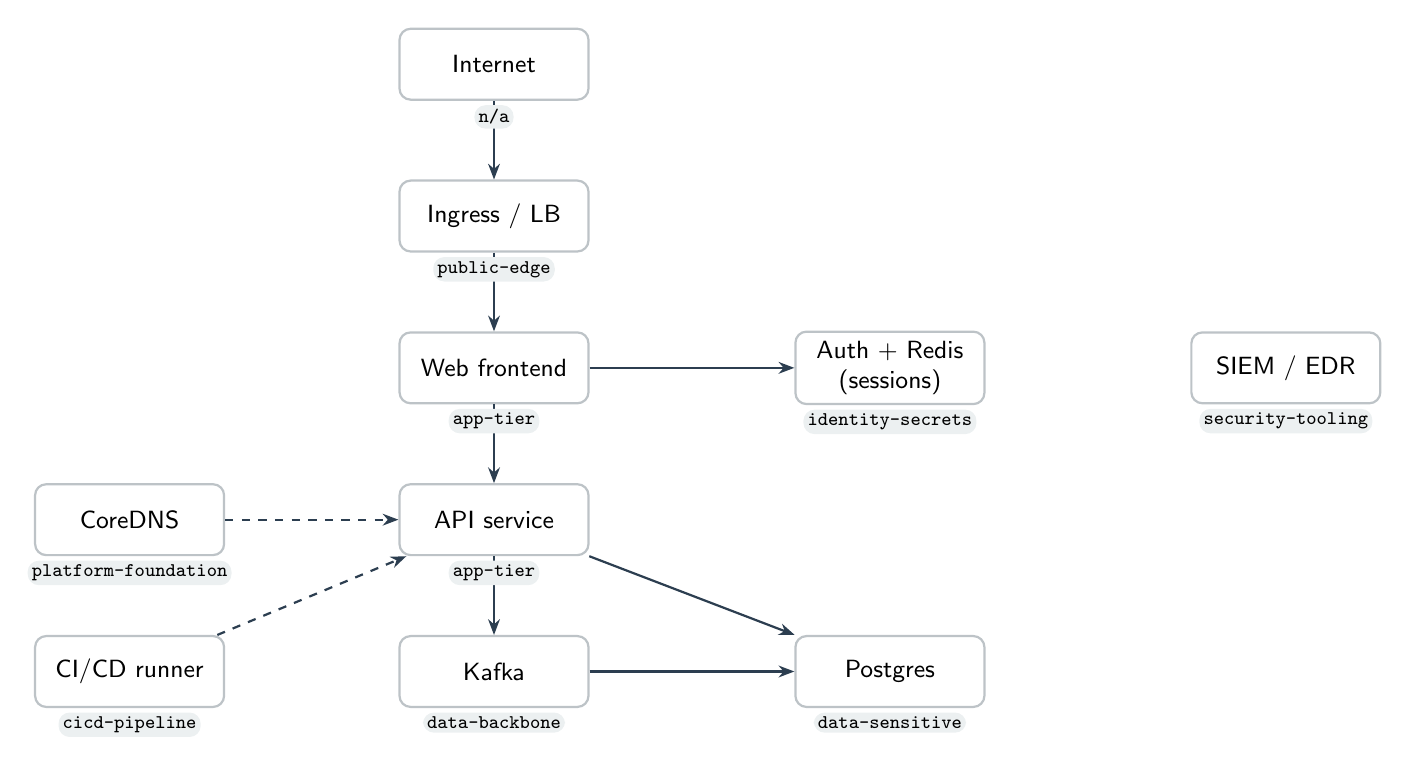
\begin{tikzpicture}[
  font=\sffamily\small,
  node distance=10mm and 14mm,
  box/.style={draw=rule,rounded corners,fill=white,minimum height=9mm,minimum width=24mm,align=center,thick},
  edge/.style={-{Stealth[length=2mm]},draw=infoblue,thick},
  tag/.style={font=\ttfamily\scriptsize,fill=tagbg,inner sep=1.5pt,rounded corners}
]
\node[box] (net) {Internet};
\node[box,below=of net] (ing) {Ingress / LB};
\node[box,below=of ing] (web) {Web frontend};
\node[box,right=26mm of web] (auth) {Auth + Redis\\(sessions)};
\node[box,below=of web] (api) {API service};
\node[box,below=of api] (kafka) {Kafka};
\node[box,right=26mm of kafka] (pg) {Postgres};
\node[box,left=22mm of api] (dns) {CoreDNS};
\node[box,left=22mm of kafka] (cicd) {CI/CD runner};
\node[box,right=26mm of auth] (siem) {SIEM / EDR};

\draw[edge] (net) -- (ing);
\draw[edge] (ing) -- (web);
\draw[edge] (web) -- (api);
\draw[edge] (web) -- (auth);
\draw[edge] (api) -- (kafka);
\draw[edge] (api) -- (pg);
\draw[edge] (kafka) -- (pg);
\draw[edge,dashed] (cicd) -- (api);
\draw[edge,dashed] (dns) -- (api);

\node[tag,below=0.5mm of net.south] {n/a};
\node[tag,below=0.5mm of ing.south] {public-edge};
\node[tag,below=0.5mm of web.south] {app-tier};
\node[tag,below=0.5mm of auth.south] {identity-secrets};
\node[tag,below=0.5mm of api.south] {app-tier};
\node[tag,below=0.5mm of kafka.south] {data-backbone};
\node[tag,below=0.5mm of pg.south] {data-sensitive};
\node[tag,below=0.5mm of dns.south] {platform-foundation};
\node[tag,below=0.5mm of cicd.south] {cicd-pipeline};
\node[tag,below=0.5mm of siem.south] {security-tooling};
\end{tikzpicture}%
}
\caption{Reference architecture; each node carries its \code{asset-archetype} tag.}
\label{fig:arch}
\end{figure}

\begin{table}[H]
\centering
\renewcommand{\arraystretch}{1.3}
\setlength{\tabcolsep}{4pt}
\footnotesize
\begin{tabular}{l l c c c c r}
\toprule
\textbf{CVE} & \textbf{Resource (archetype)} & \textbf{Classical} & \textbf{EPSS} & \textbf{Internet} & \textbf{PAIN} & \textbf{Remediation} \\
\midrule
CVE-2026-1001 & ingress \tagn{(public-edge)}        & \cellcolor{crit!25}CRITICAL & 0.97 & yes & \cellcolor{high!35}N4 & 4 days \\
CVE-2026-1002 & payments-db \tagn{(data-sensitive)} & \cellcolor{crit!25}CRITICAL & 0.94 & no  & \cellcolor{high!35}N4 & 8 days \\
CVE-2026-1003 & redis \tagn{(identity-secrets)}     & \cellcolor{high!25}HIGH     & 0.50 & no  & \cellcolor{high!35}N4 & 64 days \\
CVE-2026-1004 & kafka \tagn{(data-backbone)}        & \cellcolor{low!30}LOW       & 0.76 & no  & \cellcolor{high!35}N4 & 8 days \\
CVE-2026-1005 & web \tagn{(app-tier)}               & \cellcolor{med!35}MEDIUM    & 0.20 & yes & \cellcolor{med!35}N3 & 128 days \\
CVE-2026-1006 & coredns \tagn{(platform-foundation)}& \cellcolor{med!35}MEDIUM    & 0.08 & no  & \cellcolor{low!30}N2 & 192 days \\
\bottomrule
\end{tabular}
\caption{Sample VDR scan output (fictional data; Class~C, single-agency). PAIN is
computed from the archetype's CR/IR/AR and the CVE impact vector; the deadline is
$M[\text{C}][\text{PAIN}][\text{column}]$. Note CVE-2026-1004: a \emph{Low} vendor
severity still yields N4 because it is an availability-High DoS on a
High-availability-requirement asset (Example~3).}
\label{tab:scan}
\end{table}

\subsection{Multi-agency, Class D}
Figure~\ref{fig:archd} is a shared, multi-tenant platform serving \emph{several}
agencies at the highest assurance (Class~D). Its shared components carry more than
one agency's data, so they are tagged multi-agency (here via the cluster default,
with single-agency tenant workloads tagged as the exceptions). Table~\ref{tab:scand}
shows the result: the same families of flaws now remediate in \emph{hours}.

\begin{figure}[H]
\centering
\resizebox{\textwidth}{!}{%
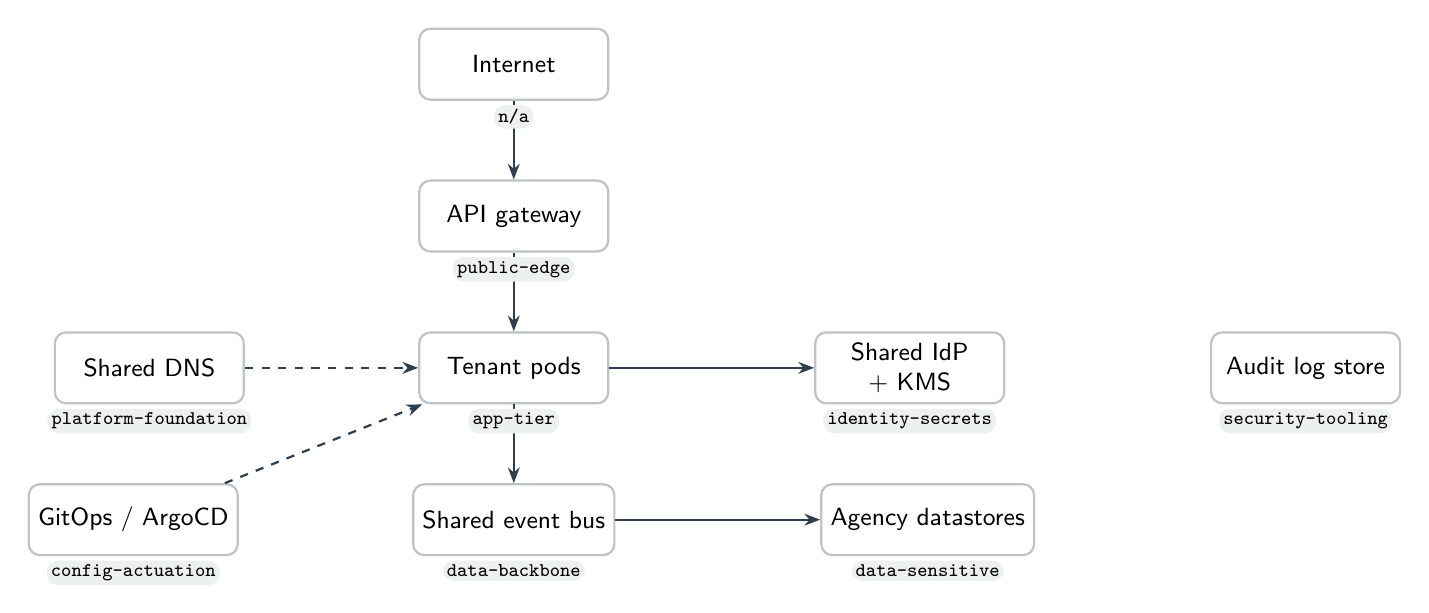
\begin{tikzpicture}[
  font=\sffamily\small,
  node distance=10mm and 14mm,
  box/.style={draw=rule,rounded corners,fill=white,minimum height=9mm,minimum width=24mm,align=center,thick},
  edge/.style={-{Stealth[length=2mm]},draw=infoblue,thick},
  tag/.style={font=\ttfamily\scriptsize,fill=tagbg,inner sep=1.5pt,rounded corners}
]
\node[box] (net) {Internet};
\node[box,below=of net] (gw) {API gateway};
\node[box,below=of gw] (app) {Tenant pods};
\node[box,right=26mm of app] (idp) {Shared IdP\\+ KMS};
\node[box,below=of app] (bus) {Shared event bus};
\node[box,right=26mm of bus] (db) {Agency datastores};
\node[box,left=22mm of app] (dns) {Shared DNS};
\node[box,left=22mm of bus] (argo) {GitOps / ArgoCD};
\node[box,right=26mm of idp] (audit) {Audit log store};

\draw[edge] (net) -- (gw);
\draw[edge] (gw) -- (app);
\draw[edge] (app) -- (idp);
\draw[edge] (app) -- (bus);
\draw[edge] (bus) -- (db);
\draw[edge,dashed] (dns) -- (app);
\draw[edge,dashed] (argo) -- (app);

\node[tag,below=0.5mm of net.south] {n/a};
\node[tag,below=0.5mm of gw.south] {public-edge};
\node[tag,below=0.5mm of app.south] {app-tier};
\node[tag,below=0.5mm of idp.south] {identity-secrets};
\node[tag,below=0.5mm of bus.south] {data-backbone};
\node[tag,below=0.5mm of db.south] {data-sensitive};
\node[tag,below=0.5mm of dns.south] {platform-foundation};
\node[tag,below=0.5mm of argo.south] {config-actuation};
\node[tag,below=0.5mm of audit.south] {security-tooling};
\end{tikzpicture}%
}
\caption{Multi-agency reference architecture; shared components serve several
agencies and are tagged multi-agency.}
\label{fig:archd}
\end{figure}

\begin{table}[H]
\centering
\renewcommand{\arraystretch}{1.3}
\setlength{\tabcolsep}{4pt}
\footnotesize
\begin{tabular}{l l c c c c r}
\toprule
\textbf{CVE} & \textbf{Resource (archetype)} & \textbf{Classical} & \textbf{EPSS} & \textbf{Internet} & \textbf{PAIN} & \textbf{Remediation} \\
\midrule
CVE-2026-2001 & gateway \tagn{(public-edge)}         & \cellcolor{crit!25}CRITICAL & 0.90 & yes & \cellcolor{crit!30}N5 & 12 hours \\
CVE-2026-2002 & shared-idp \tagn{(identity-secrets)} & \cellcolor{crit!25}CRITICAL & 0.95 & no  & \cellcolor{crit!30}N5 & 1 day \\
CVE-2026-2003 & event-bus \tagn{(data-backbone)}     & \cellcolor{low!30}LOW       & 0.80 & no  & \cellcolor{crit!30}N5 & 1 day \\
CVE-2026-2004 & agency-db \tagn{(data-sensitive)}    & \cellcolor{high!25}HIGH     & 0.40 & no  & \cellcolor{crit!30}N5 & 8 days \\
CVE-2026-2005 & tenant-pod \tagn{(app-tier)}         & \cellcolor{med!35}MEDIUM    & 0.10 & no  & \cellcolor{med!35}N3 & 64 days \\
CVE-2026-2006 & shared-dns \tagn{(platform-foundation)} & \cellcolor{med!35}MEDIUM & 0.05 & no  & \cellcolor{low!30}N2 & 192 days \\
\bottomrule
\end{tabular}
\caption{Sample VDR scan output (fictional data; Class~D, multi-agency). Multi-agency
scope escalates Disruptive/Debilitating findings, and Class~D carries the tightest
deadlines --- an internet-facing exploitable flaw on the shared edge remediates in
\textbf{12 hours} (CVE-2026-2001). CVE-2026-2003 again shows a \emph{Low} vendor
severity at N5 (availability DoS on the shared backbone). A confidentiality leak on
shared DNS (CVE-2026-2006) stays N2 --- ``Narrow'' does not escalate with scope.}
\label{tab:scand}
\end{table}

\section{Relationship to CVSS v4.0}
\label{sec:v4}
\begin{plain}
CVSS has a newer version (4.0) that changes how a flaw's impact is described and
scored. We build on the older 3.1 because it exposes the clean, transparent formula
this method depends on. Findings that only have a 4.0 score can still be handled with
a reasonable approximation, and in practice most published scores are still 3.1
today.
\end{plain}
This method is expressed in CVSS v3.1 terms because the v3.1 Environmental group
provides a closed-form Modified Impact Sub-Score (Eq.~\eqref{eq:isc}) with explicit
CR/IR/AR multipliers. CVSS v4.0 reworks impact into Vulnerable-System
(\code{VC/VI/VA}) and Subsequent-System (\code{SC/SI/SA}) metrics, removes the
\code{Scope} metric, and scores via a lookup ``MacroVector'' rather than a formula;
CR/IR/AR persist but feed that lookup. A v4.0-only finding can be \emph{approximated}
by mapping \code{VC/VI/VA} onto $C/I/A$ in Eq.~\eqref{eq:isc}, at the cost of
ignoring Subsequent-System impact. While NVD remains v3.1-dominant, an
implementation \rfckw{should} prefer the v3.1 vector and \rfckw{may} treat v4.0 via
this approximation until a native v4.0 environmental scorer is warranted.

\section{Security Considerations}
\begin{plain}
The method trusts the type-tags on each system. If someone mislabels a critical
system as trivial, its flaws will look smaller than they really are --- so the tags
must be protected like any other security setting.
\end{plain}
The method's integrity depends on the trustworthiness of two inputs: the asset
archetype tags and the VER axes (EPSS / exploitation / reachability). Tag spoofing
that \emph{lowers} an archetype is a downgrade attack; the fail-safe default and
governed calibration mitigate accidental under-classification, but tag assignment
\rfckw{should} be controlled like any other security configuration. The method does
not detect vulnerabilities; it prioritizes the output of a scanner and inherits that
scanner's coverage and accuracy.

\section{Proposal: a finer exploitability gradation (VLEV) for FedRAMP}
\label{sec:proposal}
\begin{plain}
This section is forward-looking --- a proposal we would bring to FedRAMP, not part of
the method as implemented today. Right now ``exploitability'' is a single yes/no
line. We suggest splitting it into three bands so the very tightest remediation
clocks are reserved for the flaws most likely to actually be used in the wild.
\end{plain}

\paragraph{The added inflection point.} The current model uses one EPSS cut to split
Likely-Exploitable (LEV) from Not (NLEV). We propose \emph{two} cuts and three bands:
\begin{itemize}[leftmargin=1.5em,nosep,topsep=3pt]
\item \textbf{NLEV} --- $\text{EPSS} \le 0.30$: not likely exploitable.
\item \textbf{LEV} --- $0.30 < \text{EPSS} \le 0.75$: likely exploitable.
\item \textbf{VLEV} --- $\text{EPSS} > 0.75$: \emph{very} likely exploitable.
\end{itemize}
\textbf{Observed active exploitation always maps to VLEV}, regardless of EPSS: if
CISA Vulnrichment reports \code{exploitation = active} (KEV-equivalent), the flaw is
being used \emph{now} and belongs in the most-urgent band by definition.

The payoff is twofold. The $0.30$--$0.75$ band --- today swept into the slow NLEV
column --- carries real exploitation probability and earns a tighter clock than
genuinely quiet vulnerabilities ($\le 0.30$); and the $>0.75$ / actively-exploited
flaws earn a clock tighter than today's single LEV tier provides.

\paragraph{Effect on the timelines, by Class.} VLEV introduces a new tightest column
--- roughly half the current LEV+IRV deadline, floored at 12 hours. The existing LEV
deadlines carry over to the new $0.30$--$0.75$ band, and NLEV (now $\le 0.30$) keeps
its relaxed deadline. The proposed VLEV+IRV floor:

\begin{table}[H]
\centering
\footnotesize
\renewcommand{\arraystretch}{1.2}
\begin{tabular}{l ccc}
\toprule
& \multicolumn{3}{c}{\textbf{Proposed VLEV+IRV deadline, days --- (current LEV+IRV)}} \\
\cmidrule(lr){2-4}
\textbf{PAIN} & \textbf{Class A/B} & \textbf{Class C} & \textbf{Class D} \\
\midrule
N5 & 2 \,(4)   & 1 \,(2)   & 0.5 \,(0.5) \\
N4 & 4 \,(8)   & 2 \,(4)   & 1 \,(2) \\
N3 & 16 \,(32) & 8 \,(16)  & 4 \,(8) \\
N2 & 48 \,(96) & 24 \,(48) & 12 \,(24) \\
\bottomrule
\end{tabular}
\caption{Proposed VLEV+IRV remediation floor by Class (current LEV+IRV in
parentheses); days, $0.5 = 12$ hours. The new LEV band ($0.30$--$0.75$ EPSS) inherits
today's LEV deadlines; NLEV ($\le 0.30$) is unchanged; the NIRV variants relax by the
same factor as today. PAIN-1 still carries no FedRAMP deadline.}
\end{table}

\noindent Net effect: actively-exploited and $>0.75$-EPSS flaws on high-PAIN,
internet-reachable assets compress toward \emph{hours} at the stricter Classes, while
the broad $0.30$--$0.75$ middle band --- previously treated as ``not likely'' ---
moves onto a real clock. Mechanically this is additive: the remediation matrix is
already a config-driven \code{[Class][PAIN][column]} lookup, so VLEV is one more
column, not a redesign.

\section{Conclusion}
FedRAMP Rev5 VDR/VER specifies the vocabulary and the axes of vulnerability
prioritization but leaves the classifier unspecified. That classifier need not be
invented: the CVSS Environmental metric group already encodes ``re-weight impact by
what is at stake,'' which is precisely the agency-impact question. By assigning each
asset its CR/IR/AR --- via archetypes or any other systematic scheme the CSP owns
--- and evaluating the two VER axes, a provider obtains a deterministic, auditable,
and standards-grounded PAIN and remediation deadline for every finding. We offer the
example archetype catalog not as a standard but as an existence proof; we encourage
each CSP to publish its own.

\appendix
\section{Example archetype catalog}
\label{app:catalog}
Illustrative only (see Section~\ref{sec:archetypes}).

\begin{table}[H]
\centering
\renewcommand{\arraystretch}{1.2}
\footnotesize
\setlength{\tabcolsep}{5pt}
\begin{tabular}{l l c c c >{\raggedright\arraybackslash}p{0.34\textwidth}}
\toprule
\textbf{Archetype} & \textbf{Lens} & \textbf{CR} & \textbf{IR} & \textbf{AR} & \textbf{Typical members} \\
\midrule
\code{cicd-pipeline}      & control & H & H & H & build/deploy runners, artifact signing, registries \\
\code{orchestrator}       & control & H & H & H & control plane, etcd, scheduler, coordination \\
\code{config-actuation}   & control & H & H & H & IaC/GitOps, schema registry, admin/migration \\
\code{identity-secrets}   & control & H & H & H & IdP/SSO, KMS, secrets managers, session stores \\
\code{security-tooling}   & control & H & H & M & scanners, SIEM, EDR, runtime security \\
\code{change-record}      & control & M & M & M & ITSM/ticketing (record only) \\
\code{platform-foundation}& control & L & H & H & DNS, NTP, service discovery, L4 internal LBs (metadata only) \\
\code{data-sensitive}     & data    & H & H & H & PII/CUI datastores \\
\code{data-backbone}      & data    & H & H & H & queues, brokers, the system-of-record DB \\
\code{app-tier}           & data    & M & M & H & stateless services, APIs, UIs, caches \\
\code{batch-analytics}    & data    & M & M & L & ETL, reporting, analytics jobs \\
\code{public-edge}        & data    & L & L & H & load balancers, public web, ingress \\
\code{internal-tooling}   & data    & L & L & L & dashboards, metrics/log agents \\
\code{dev-test}           & data    & L & L & L & non-production \\
\midrule
\code{unclassified}       & ---     & H & H & H & fail-safe default for untagged assets \\
\bottomrule
\end{tabular}
\end{table}

\section{Remediation deadline matrices}
\label{app:matrix}
Days; $0.5 = 12$ hours. Columns in order LEV+IRV / LEV+NIRV / NLEV. PAIN-1 has no
FedRAMP deadline (any class). Values illustrative of a representative VDR-TFR-PVR
profile.

\begin{table}[H]
\centering
\footnotesize
\renewcommand{\arraystretch}{1.2}
\begin{tabular}{l ccc @{\hspace{2em}} ccc @{\hspace{2em}} ccc}
\toprule
& \multicolumn{3}{c}{\textbf{Class A / B}} & \multicolumn{3}{c}{\textbf{Class C}} & \multicolumn{3}{c}{\textbf{Class D}} \\
\cmidrule(lr){2-4}\cmidrule(lr){5-7}\cmidrule(lr){8-10}
\textbf{PAIN} & L+I & L+N & NLEV & L+I & L+N & NLEV & L+I & L+N & NLEV \\
\midrule
N5 & 4  & 8   & 32  & 2  & 4   & 16  & 0.5 & 1  & 8  \\
N4 & 8  & 32  & 64  & 4  & 8   & 64  & 2   & 8  & 32 \\
N3 & 32 & 64  & 192 & 16 & 32  & 128 & 8   & 16 & 64 \\
N2 & 96 & 160 & 192 & 48 & 128 & 192 & 24  & 96 & 192 \\
\bottomrule
\end{tabular}
\end{table}

\section{Explicit design opinions (calibratable choices)}
\label{app:opinions}
\begin{plain}
Everything in this section is a \emph{judgment call} we made --- not something
FedRAMP or CVSS dictates. We collect them in one place so reviewers can challenge
each one, and so any adopter knows exactly which dials are theirs to turn. None of
these is load-bearing for the \emph{method}; they are the parameters the method runs
on.
\end{plain}

The method deliberately separates standardized arithmetic (Section~\ref{sec:math})
from a small set of explicit opinions. Each item below states the value we use, why,
and the fact that an implementation \rfckw{may} change it.

\begin{enumerate}[leftmargin=1.7em]
\item \textbf{PAIN word thresholds $(\theta_1,\theta_2,\theta_3) = (0.25,\,0.55,\,0.80)$.}
  The cut points that turn the impact scalar $S$ into
  Minimal/Narrow/Disruptive/Debilitating (Eq.~\ref{eq:word}). This is the single most
  consequential opinion --- it sets where a finding crosses an N-level boundary. The
  values should reproduce senior-analyst triage on a back-tested sample; an adopter
  \rfckw{should} re-calibrate against its own rated findings and \rfckw{must} treat
  the result as governed configuration.
\item \textbf{EPSS Likely-Exploitable threshold $\theta_{\text{epss}} = 0.70$.}
  The EPSS probability at or above which a finding is treated as LEV
  (Section~\ref{sec:remediation}). Higher means fewer findings on the fast track;
  FedRAMP leaves the framework to the provider.
\item \textbf{LEV is a union, not a blend.} A finding is Likely Exploitable if
  EPSS $\ge \theta_{\text{epss}}$ \emph{or} exploitation is observed ``active'' ---
  whichever fires, with no weighting between them.
\item \textbf{Internet-reachability counts edge authentication as a mitigation.} We
  define IRV as ``fronted by a public load balancer/route whose edge does not enforce
  authentication.'' A route gated by a native identity-aware proxy (or equivalent) is
  treated as \emph{not} internet-reachable, on the view that an unauthenticated
  attacker cannot reach the vulnerable surface. An adopter wanting a stricter posture
  \rfckw{may} count any public route as IRV regardless of edge authentication.
\item \textbf{Impact-only severity, normalized by $0.915$.} We take CVSS's
  \emph{Modified Impact Sub-Score} and rescale it to $[0,1]$ (Eq.~\ref{eq:s}) rather
  than computing the full 0--10 environmental score. PAIN is about \emph{impact on the
  asset}, so we intentionally drop the exploitability half of the base score (and the
  $6.42$ coefficient) from the severity term; exploitability re-enters separately as
  the LEV/IRV remediation columns.
\item \textbf{Technical impact is a floor, not the primary signal.} ``technical
  impact = total'' raises each \emph{in-scope} CVSS dimension to High; it never
  invents impact on a dimension the CVE marks None, and ``partial''/absent leaves the
  vector unchanged. (An earlier draft made technical impact primary with CVSS as the
  fallback; we reversed that.)
\item \textbf{CISA Vulnrichment as the authoritative enrichment source.} The
  exploitation state (active / PoC / none) and the technical impact (total / partial)
  are taken from \emph{CISA Vulnrichment}, CISA's Authorized Data Publisher (ADP)
  enrichment of CVE records. Deferring to an ADP's assessment --- rather than a
  bespoke or purely commercial judgment --- keeps these inputs authoritative and
  governed; an adopter \rfckw{may} substitute or augment with another source (a
  vendor SSVC decision, a commercial threat-intelligence feed, or the CISA KEV
  catalog). EPSS, by contrast, supplies the statistical exploitation \emph{likelihood}
  (item~2); the two are complementary.
\item \textbf{Scope is purely hierarchical.} An asset is multi-agency only if it ---
  or its namespace, or the cluster default --- is tagged so (most-specific wins);
  there is no automatic per-archetype escalation. (An earlier draft auto-escalated
  ``shared-infrastructure'' archetypes to multi-agency; we removed that in favor of
  explicit, operator-controlled tagging.)
\item \textbf{``Archetype'', not ``type''.} We classify assets by their
  \emph{role/usage pattern}, not their intrinsic kind, and the label reflects that:
  the same software lands in different archetypes by how it is used (an in-memory
  store is \code{app-tier} as a cache, \code{identity-secrets} as a session store,
  \code{data-backbone} as a broker). ``Type'' would wrongly suggest an intrinsic
  property of the software and collides with overloaded terms (e.g.\ Kubernetes
  Service \code{type}); ``archetype'' names the pattern an asset matches in the
  estate. An adopter \rfckw{may} rename the label, but the role-not-kind semantics
  should be preserved.
\item \textbf{Fail-safe defaults to conservative High.} An unclassified asset defaults
  to CR/IR/AR all High so it scores loudly, rather than to a low default. ``Unknown''
  is treated as serious until classified.
\item \textbf{CVSS v3.1, not v4.0.} We build on v3.1's closed-form environmental
  formula; v4.0 findings are approximated by mapping VC/VI/VA onto $C/I/A$
  (Section~\ref{sec:v4}).
\item \textbf{The archetype catalog and its CR/IR/AR values
  (Appendix~\ref{app:catalog}).} Illustrative only --- each CSP \rfckw{should} derive
  its own from its system categorization.
\item \textbf{The remediation deadline values (Appendix~\ref{app:matrix}).}
  Representative of a plausible VDR-TFR-PVR profile; the authoritative day counts
  follow FedRAMP and the provider's Certification-Class commitments.
\end{enumerate}

\end{document}
